\documentclass[12pt]{report}
\usepackage{fontspec}
\usepackage[14pt]{extsizes}
\usepackage[english, russian]{babel} 
\defaultfontfeatures{Ligatures={TeX},Renderer=Basic} 
\setmainfont[Ligatures={TeX,Historic}]{Times New Roman}
\usepackage{setspace} % полуторный интервал

\usepackage{caption}

\usepackage{graphicx}

\usepackage[left=2cm, right=2cm, top=2cm, bottom=2.5cm]{geometry}
\usepackage{hyperref}
\usepackage{amsmath,amsfonts,amssymb,amsthm} 

\usepackage{titlesec, blindtext, color} % подключаем нужные пакеты
\definecolor{gray75}{gray}{0.75} % определяем цвет
\newcommand{\hsp}{\hspace{20pt}} % длина линии в 20pt
\titleformat{\chapter}[hang]{\Huge\bfseries}{\thechapter\hsp\textcolor{gray75}{|}\hsp}{0pt}{\Huge\bfseries}

\usepackage{listings}
% Для листинга кода:
\lstset{ 
	language=[Sharp]C,                 % выбор языка для подсветки (здесь это С)
	basicstyle=\small\sffamily, % размер и начертание шрифта для подсветки кода
	numbers=left,               % где поставить нумерацию строк (слева\справа)
	numberstyle=\tiny,           % размер шрифта для номеров строк
	stepnumber=1,                   % размер шага между двумя номерами строк
	numbersep=5pt,                % как далеко отстоят номера строк от подсвечиваемого кода
	showspaces=false,            % показывать или нет пробелы специальными отступами
	showstringspaces=false,      % показывать или нет пробелы в строках
	showtabs=false,             % показывать или нет табуляцию в строках
	frame=single,              % рисовать рамку вокруг кода
	tabsize=2,                 % размер табуляции по умолчанию равен 2 пробелам
	captionpos=t,              % позиция заголовка вверху [t] или внизу [b] 
	breaklines=true,           % автоматически переносить строки (да\нет)
	breakatwhitespace=false, % переносить строки только если есть пробел
}

\begin{document}
	
	%\def\chaptername{} % убирает "Глава"
	\begin{titlepage}
		\begin{table}[ht]
			\centering
			\begin{tabular}{|c|p{400pt}|} 
				\hline
				\begin{tabular}[c]{@{}c@{}} 
\includegraphics[scale=0.40]{source/EmblemBMSTU} \\\end{tabular} &
				\footnotesize\begin{tabular}[c]{@{}c@{}}\textbf{Министерство~науки~и~высшего~образования~Российской~Федерации}\\\textbf{Федеральное~государственное~бюджетное~образовательное~учреждение}\\\textbf{~высшего~образования}\\\textbf{«Московский~государственный~технический~университет}\\\textbf{имени~Н.Э.~Баумана}\\\textbf{(национальный~исследовательский~университет)»}\\\textbf{(МГТУ~им.~Н.Э.~Баумана)}\\\end{tabular}  \\
				\hline
			\end{tabular}
		\end{table}
		\noindent\rule{\textwidth}{4pt}
		\noindent\rule[14pt]{\textwidth}{1pt}
		\hfill 
		\noindent
		\makebox{ФАКУЛЬТЕТ~}%
		\makebox[\textwidth][l]{\underline{~~~~«Информатика и системы управления»~~~~~~~~~~~~~~~~~~~~~~~~~~~~~~~~~~~~~~~~~~~~}}%
		\\
		\noindent
		\makebox{КАФЕДРА~}%
		\makebox[\textwidth][l]{\underline{~~~~~~«Программное обеспечение ЭВМ и информационные технологии»~}}%
		\\
		
		
		\begin{center}
			\vspace{3cm}
			{\bf\huge Отчёт\par}
			{\bf\Large по лабораторной работе № 3\par}
			\vspace{0.5cm}
		\end{center}
		
		
		\noindent
		\makebox{\large{\bf Название:}~~~}
		\makebox[\textwidth][l]{\large\underline{~Алгоритмы сортировки~}}\\
		
		\noindent
		\makebox{\large{\bf Дисциплина:}~~~}
		\makebox[\textwidth][l]{\large\underline{~Анализ алгоритмов~}}\\
		
		\vspace{1.5cm}
		\noindent
		\begin{tabular}{l c c c c c}
			Студент      & ~ИУ7-55Б~               & \hspace{3.5cm} & \hspace{3.5cm}                 & &  Д.О. Склифасовский \\\cline{2-2}\cline{4-4} \cline{6-6} 
			\hspace{3cm} & {\footnotesize(Группа)} &                & {\footnotesize(Подпись, дата)} & & {\footnotesize(И.О. Фамилия)}
		\end{tabular}
		
		\vspace{1cm}
		
		\noindent
		\begin{tabular}{l c c c c}
			Преподователь & \hspace{6cm}   & \hspace{3.5cm}                 & & ~~~~~~ Л.Л. Волкова ~~~~~~\\\cline{3-3} \cline{5-5} 
			\hspace{3cm}  &                & {\footnotesize(Подпись, дата)} & & {\footnotesize(И.О. Фамилия)}
		\end{tabular}
		
		\begin{center}	
			\vfill
			\large \textit {Москва, 2020}
		\end{center}
		
		\thispagestyle {empty}
		\pagebreak
	\end{titlepage}
	\restoregeometry
	
	\tableofcontents
	\onehalfspacing
	\newpage
	\chapter*{Введение}
	\addcontentsline{toc}{chapter}{Введение}
	Цель работы: изучение алгоритмов сортировки массивов. В данной лабораторной работе рассматриваются 3 алгоритма:
	\begin{enumerate}
		\item[1)] сортировка пузырьком;
		\item[2)] сортировка шейкером;
		\item[3)] сортировка вставками. 
	\end{enumerate}
	\noindent Также требуется изучить рассчет сложности алгоритмов. В ходе лабораторной работы необходимо:
	\begin{enumerate}
		\item[1)] изучить алгоритмы сортировки;
		\item[2)] дать теоритическую оценку сортировок пузырьком, шейкером и вставками;
		\item[3)] реализовать три алгоритма сортировки на одном из языков программирования;
		\item[4)] сравнить алгоритмы сортировки.    
	\end{enumerate}

	\chapter{Аналитическая часть}
	В данном разделе представлено описание алгоритмов сортировки массивов.
	\section{Сортировка пузырьком}
	Сортировка пузырьком — один из самых известных алгоритмов сортировки. Здесь нужно последовательно сравнивать значения соседних элементов и менять числа местами, если предыдущее оказывается больше последующего. Таким образом элементы с большими значениями оказываются в конце списка, а с меньшими остаются в начале.
	\par\noindent Этот алгоритм считается учебным и почти не применяется на практике из-за низкой эффективности: он медленно работает на тестах, в которых маленькие элементы (их называют «черепахами») стоят в конце массива. Однако на нём основаны многие другие методы, например, шейкерная сортировка и сортировка расчёской.
	\section{Сортировка шейкером}
	Шейкерная сортировка отличается от пузырьковой тем, что она двунаправленная: алгоритм перемещается не строго слева направо, а сначала слева направо, затем справа налево.
	\section{Сортировка вставками}
	При сортировке вставками массив постепенно перебирается слева направо. При этом каждый последующий элемент размещается так, чтобы он оказался между ближайшими элементами с минимальным и максимальным значением.
	\section{Вывод}
	Было представлено описание алгоритмов сортировки массивов. В основном все алгоритмы сортировок основаны на алгоритме сортировки пузырьком.

	\chapter{Конструкторская часть}
	В данном разделе представлены съемы разработанных алгоритмов. Также оценивается трудоемкость алгоритмов.
	\section{Разработка алгоритмов}
	На \hyperref[Schema1]{рисунке 1} изображена схема алгоритма сортировки пузырьком.
	\begin{figure}[h!]\label{Schema1}
		\center{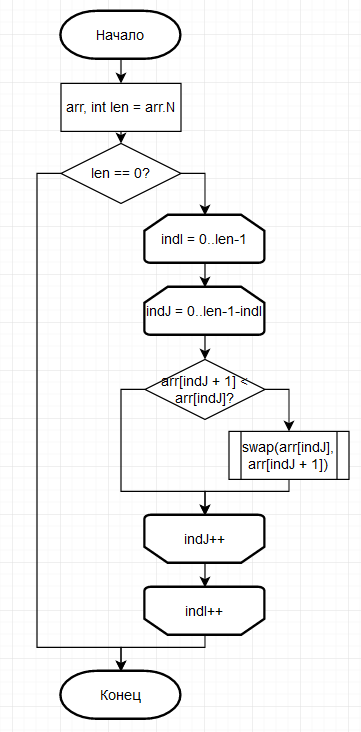
\includegraphics[scale=0.95]{source/Schema1.png}}
		\caption*{Рисунок 1. Схема алгоритма сортировки пузырьком}
	\end{figure}
	\newpage
	На \hyperref[Schema2]{рисунке 2} изображена схема алгоритма сортировки шейкером.
	\begin{figure}[h!]\label{Schema2}
		\center{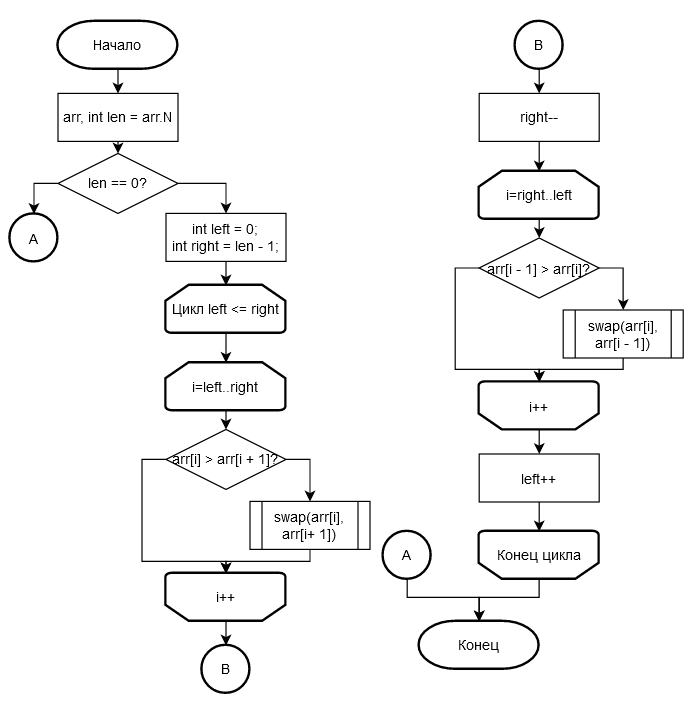
\includegraphics[scale=0.95]{source/Schema2.png}}
		\caption*{Рисунок 2. Схема алгоритма сортировки шейкером}
	\end{figure}
	\newpage
	На \hyperref[Schema3]{рисунке 3} изображена схема алгоритма сортировки вставками.
	\begin{figure}[h!]\label{Schema3}
		\center{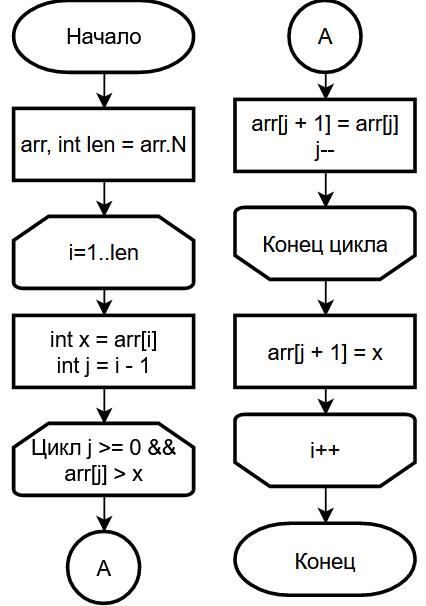
\includegraphics[scale=0.95]{source/Schema3.png}}
		\caption*{Рисунок 1. Схема алгоритма сортировки вставками}
	\end{figure}
	\newpage

	\section{Модель трудоемкости}
	Модель трудоемкости для оценки алгоритмов:
	\begin{enumerate}
		\item[1)] стоимость базовых операций единица:\par
		$=,+,*,\simeq,<,>,\geq,\leq,==,!=,[],+=,-=,*=,/=,++,--$;
		\item[2)] стоимость цикла:\par
		$f_{for}=f_{init}+f_{comp}+M(f_{body}+f_{increment}+f_{comp})$\par
		Пример: $for(i=0,i<M;i++){/* body */}$\par
		Результат: $2 + M(2+f_{body})$;
		\item[3)] стоимость условного оператора\par
		Пусть goto (переход к одной из ветвей) стоит 0, тогда\par
		\begin{displaymath}
			f_{f} = \left\{ \begin{array}{l l}
				min(f_{A},f_{B}), & \textrm{лучший случай}\\
				max(f_{A},f_{B}), & \textrm{худший случай}\\
			\end{array} \right.
		\end{displaymath}
		\item[4)] операция обращения к ячейки матрицы [i, j] имеет трудоёмкость равную двум.
	\end{enumerate}

	\section{Оценка трудоемкости алгоритмов сортировки}
	Оценим трудоемкость алгоритмов.
	\subsection{Сортировка пузырьком}
	Лучший случай (массив отсортирован): 
	\begin{displaymath}
		2 + 1 + 1 + 2 + (len-1)(1 + 2 + )
	\end{displaymath}

	\section{Вывод}
	В данном разделе были рассмотрены схемы алгоритмов сортировки массива, введена модель оценки трудоемкости алгоритма и были рассчитаны трудоемкости алгоритмов.

	\chapter{Технологическая часть}
	В данном разделе даны общие требования к программе, средства реализации и реализация алгоритмов.

	\section{Общие требования к программе}
	\textbf{Требования к вводу:}
	\begin{enumerate}
		\item[1)] вводится размер массива;
		\item[2)] вводятся или автоматически генерируется массив. 
	\end{enumerate}
	\begin{enumerate}
		\item[1)] при вводе неправильных размеров массива программа не должна завершаться аварийно;
		\item[2)] должна выполняться корректная сортировка массива. 
	\end{enumerate}

	\section{Средства реализации}
	В качестве языка программирования был выбран C\#, так как я знаком с данным языком программирования, имею представление о способах тестирования программы.
	\noindent Средой разработки Visual Studio.
	\noindent Для замеров процессорного времени используется функция Stopwatch.

	\section{Сведения о модулях программы}
	Программа состоит из:
	\begin{enumerate}
		\item[1)] Program.cs - главный файл программы, в котором располагается точка входа в программу;
		\item[2)] Array.cs - файл класса Array;
		\item[3)] Sort.cs - файл класса Sort. В нем находятся алгоритмы сортировки массивов.
	\end{enumerate}

	\section{Листинг кода программы}
	\begin{lstlisting}[label=Array,caption=Класс Array для работы с массивами]
		class Array
		{
			private int[] array;
			private int n;
			public Array() { }

			public Array(int n)
			{
				this.n = n;
				array = new int[n];
			}

			public int N
			{
				get { return n; }
				set { if (value > 0) n = 0; }
			}

			public int this[int i]
			{
				get { return array[i]; }
				set { array[i] = value; }
			}

			public void Copy(Array arr)
			{
				for (int i = 0; i < n; i++)
				{
					arr[i] = array[i];
				}
			}

			public void Read()
			{
				for (int i = 0; i < n; i++)
				{
					Console.Write(array[i] + "\t");
				}
				Console.WriteLine();
			}

			public void Fill()
			{
				Random rand = new Random();
				for (int i = 0; i < n; i++)
				{
					array[i] = rand.Next(100);
				}
			}
		}
	\end{lstlisting}
	\begin{lstlisting}[label=BubleSort,caption=Алгоритм сортировки пузырьком]
		public static void BubbleSort(Array arr)
        {
            int len = arr.N;
            if (len == 0)
            {
                return;
            }

            for (int indI = 0; indI + 1 < len; indI++)
            {
                for (int indJ = 0; indJ + 1 < len - indI; indJ++)
                {
                    if (arr[indJ + 1] < arr[indJ])
                    {
                        int tmp = arr[indJ];
                        arr[indJ] = arr[indJ + 1];
                        arr[indJ + 1] = tmp;
                    }
                }
            }
        }
	\end{lstlisting}
	\begin{lstlisting}[label=ShakerSort,caption=Алгоритм сортировки шейкером]
		public static void ShakerSort(Array arr)
        {
            int len = arr.N;
            if (len == 0)
            {
                return;
            }
            int left = 0;
            int right = len - 1;
            while (left <= right)
            {
                for (int i = left; i < right; i++)
                {
                    if (arr[i] > arr[i + 1])
                    {
                        int tmp = arr[i];
                        arr[i] = arr[i + 1];
                        arr[i + 1] = tmp;
                    }
                }
                right--;

                for (int i = right; i > left; i--)
                {
                    if (arr[i - 1] > arr[i])
                    {
                        int tmp = arr[i];
                        arr[i] = arr[i - 1];
                        arr[i - 1] = tmp;
                    }
                }
                left++;
            }
        }
	\end{lstlisting}
	\begin{lstlisting}[label=InsertionSort,caption=Алгоритм сортировки вставками]
		public static void InsertionSort(Array arr)
        {
            int len = arr.N;
            if (len == 0)
            {
                return;
            }
            for (int i = 1; i < len; i++)
            {
                int x = arr[i];
                int j = i - 1;
                for (; j >= 0 && arr[j] > x; j--)
                {
                    arr[j + 1] = arr[j];
                }
                arr[j + 1] = x;
            }
        }
	\end{lstlisting}

	\section{Вывод}
	В данном разделе были представлены сведения о модулях программы, а также реализованы три алгоритма сортировки массивов.

	\chapter{Экспериментальная часть}
	В данном разделе представлены результаты работы программы и приведен анализ времени работы каждого из алгоритмов.
	
	\section{Примеры работы программы}

\end{document}

